\documentclass{amsart}
% option ``report'' puts title on separate page

\usepackage{amsmath}
\usepackage[pdftex]{graphicx}

\begin{document}

\title{Monte Carlo Radiation Transport}
\author{Jackie Villadsen}
\date{\today}
\maketitle

\section{Motivation}

Radiative transport is an important mechanism in a wide variety of
astrophysical situations.  At high temperatures (for non-relativistic
electrons), the dominant source of opacity is Thomson scattering off of electrons, which is independent of wavelength and does not destroy photons.  
Even in situations where absorption is important, scattering can be used
as a rough proxy for absorption then re-emission.
This code simulates the path of photons emitted by a central star and then undergoing isotropic scatterings, in order to
understand the distribution of times to escape from a surrounding nebula,
and the angular distribution of intensity due to that nebula.
The code is applied to the examples of shock breakout in supernovae and
planetary nebulae.

\subsection{Planetary Nebulae}
After the Asymptotic Giant Branch (AGB) phase, a star has a degenerate carbon-oxygen core and a hydrogen shell, with nuclear burning occurring in the shell.  In this state, the star pulsates strongly, blowing off the outer layers of its atmosphere.  As the outer layers of the star are ejected, the high-temperature core (a white dwarf) is revealed, blasting the ejecta with ionizing photons.  These glowing, ionized ejecta are known as a planetary nebula.  The central white dwarf cools via radiation, and eventually its effective temperature drops low enough that it no longer produces enough ionizing photons to keep the planetary nebula ionized, and so the planetary nebula recombines and fades away.  The entire lifetime of a planetary nebula is only of order 10,000 years, so they are very rare objects.

Planetary nebulae come in a variety of different configurations.  Only a fraction of them are spherical.  They may also have clumpy distributions due to the different waves of ejected matter during the stellar pulsations.  Radiative transfer by isotropic scattering can be used as a proxy for ionization and recombination (with isotropic emission) in order to determine the morphology of planetary nebulae with a range of density distributions.

\subsection{Shock Breakout}
Supernovae progenitors are very massive, very extended stars.  The largest
of these, red supergiants (RSGs) can be roughly 1000$R_\odot$ in size, so that the light travel time from the center to the edge is of order an hour.  
Thus, when the process of core collapse starts in the center of the star, there is no visible sign of it for at least an hour.  This is compounded by the fact that radiation is trapped inside the optically thick star, and swept along by the shock at a speed of order $v_s\sim10,000$ km/s $\sim c/30$, so it will be quite a few hours before the first supernova radiation becomes visible.

When the shock nears the edge of the progenitor, the photon diffusion timescale to the edge of the star becomes shorter than the time for the shock to travel that distance.
At this point, the photons diffuse out and the first radiation from the supernova becomes visible.  The duration of this initial burst of X-ray photons that have escaped from the shock front, known as ``shock breakout,'' is determined by the diffusion timescale plus the light travel time across the radius of the star (since the light from the edges of the star travels further to reach the observer than the light from the center of the star).

The photons start to diffuse outward through atmosphere of thickness $dR$ when the photon diffusion timescale with mean free path $l$ is roughly equal to the time for the shock to escape at velocity $v_s$:
\begin{equation}
	\frac{dR^2}{lc} = \frac{dR}{v_s}
\end{equation}
The optical depth $\tau=dR/l$ so shock breakout starts when
$\tau=c/v_s{\sim}30$.

The light travel time $t_l=R_*/c$ determines the duration of shock breakout when $R_*>dR^2/l=\tau{dR}$, whereas the photon diffusion timescale dominates for smaller $R_*$.  This project assumes the same $v_s$ for all progenitors,
and thus the same $\tau$.  $dR$ is the scale height of the density distribution of the outer layer of the progenitor - approximately $R_*/50$ for a stellar atmosphere, or $R_*/2$ for a stellar wind - so $dR{\propto}R_*$ in both cases.  Since both the diffusion timescale and the light travel time are proportional to $R_*$ in the simple model used here, the simulations discussed below should show this property.  In more realistic models, such as discussed in Calzavara \& Matzner (2004), the diffusion timescale is no longer linear in $R_*$, leading to a range of progenitor radii for which light travel time dominates, and a range for which diffusion time dominates.

\section{1D Code}
\subsection{Outline of Code}
The steps taken by the code to simulate 1D radiation transport are:
\begin{enumerate}
\item Sample a density distribution from $R_{inner}$ to $R_{outer}$, where $R_{inner}$ may be larger than $R_*$ to allow for a central cavity around the star. Calculate mean free path at all R.
\item Track a large number of photons as they move through the nebula.
\begin{enumerate}
\item Photon starts at $R_{inner}$.
\item At location of photon, interpolate to obtain mean free path $\lambda$.
\item Use Monte Carlo sampling of an exponential distribution with mean free path $\lambda$ to obtain a step size.
\item Move to new location determined by step size.
\item Generate a random direction (isotropic scattering), which in 1D is + or -.
\item Repeat stepping and scattering procedure until the photon either emerges from the nebular ($r>R_{inner}$) or is absorbed by striking the star.
\end{enumerate}
The code tracks the position history of every photon, as well as the total time passed before the photon emerges from the nebula.
\end{enumerate}
\subsubsection{Setting Up Density Grid Based on Optical Depth}
The code allows the user to set the optical depth $\tau$ from $R_{inner}$ to $R_{outer}$.  The code first solves for $\left<\rho\right>$ using:
\begin{equation}
	\tau = \int_{R_{inner}}^{R_{outer}} \kappa \rho(r) dr
             = \kappa \left<\rho\right> (R_{outer} - R_{inner})
\end{equation}
which assumes a constant value of $\kappa=0.2$ cm$^2$/g.

Based on user selection, the code then computes one of the following
density distributions (which are normalized to have average value $\left<\rho\right>$,
integrated along a radial line, and therefore optical depth $\tau$).  In
these equations, $\Delta{R}=R_{outer}-R_{inner}$.
\begin{itemize}
\item Flat:
\begin{equation}
	\rho(r) = \left<\rho\right>
\end{equation}
\item Power law ($\rho{\propto}r^{-a}$), where $f=R_{outer}/R_{inner}$:
\begin{equation}
	\rho(r) = \left<\rho\right> \left( \frac{(a-1) (f-1)}
		  {1 - f^{-(a-1)}} \right)
		  \left(\frac{R_{inner}}{r}\right)^{-a}
\end{equation}
An $r^{-a}$ power law yields an atmosphere scale height $H{\approx}R_*/a$.
\item ``Clumpy'' distribution with N clumps (represented by a sinusoid with N periods in length $\Delta{R}$):
\begin{equation}
	\rho(r) = \left<\rho\right> \left( 1 - \sin\left[\frac{2\pi N}{\Delta{R}}(r-R_{inner}) \right] \right)
\end{equation}
\end{itemize}
Figure \ref{fig:densities} shows examples of each of these density profiles.

\subsubsection{Monte Carlo Sampling of Step Size}

\begin{figure}[h]
  \begin{center}
     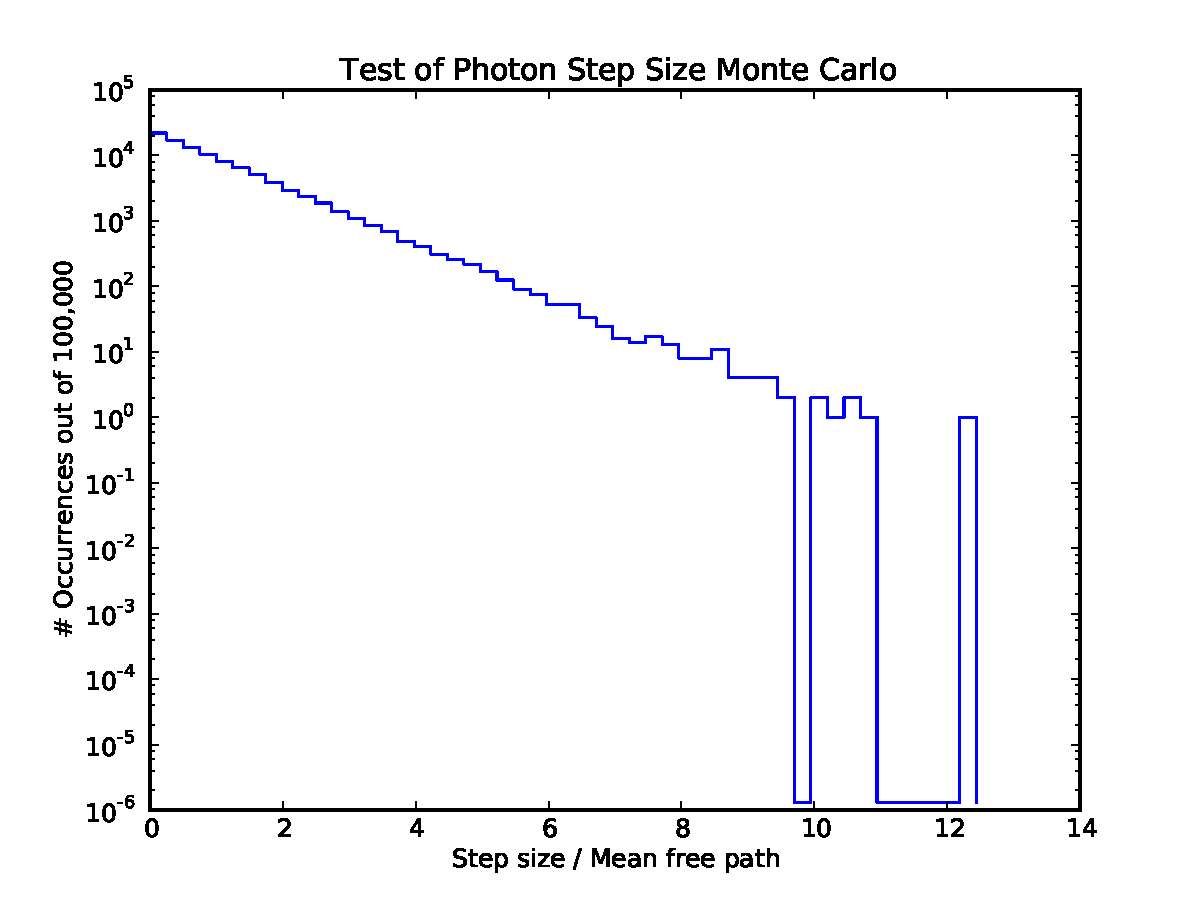
\includegraphics[width=\textwidth]{mctest}
  \end{center}
  \caption{Histogram of 100,000 step sizes generated from an exponential
distribution with mean free path $\lambda$.  The variation at high
step size is due to undersampling.  The distribution appears linear when
displayed with an exponential y-axis, so it is an exponential distribution.}
  \label{fig:mctest}
\end{figure}

In a region with mean free path $\lambda$, the cumulative probability
that a photon will scatter before traveling distance $l$ is:
\begin{equation}
	P(l|\lambda) = 1 - e^{-l/\lambda}
\end{equation}
and the differential probability of scattering after traveling
a distance between $l$ and $l+dl$
is:
\begin{equation}
	p(l|\lambda) = \frac{1}{\lambda}e^{-l/\lambda}
\end{equation}

To sample from the distribution $p(l|\lambda)$, I generate a random
number $y$ between 0 and 1, and set it equal to the cumulative
probability, then solve for $l$:
\begin{equation}
	l = -\lambda \ln (1-y)
\end{equation}

To verify that this yields an exponential distribution with mean $\left<l\right>=\lambda$, I used this method to generate N=100,000 step sizes for a
mean free path of $\lambda=1$.  Figure \ref{fig:mctest} shows the
resulting exponential distribution of step sizes, and the mean $l$
generated by this method was $\left<l\right>=1.002$, so $\left<l\right>=\lambda$ to within an error of order $1/\sqrt{N}$.

\subsection{Test 1: Mean Distance Traveled}

\begin{figure}[h]
  \begin{center}
     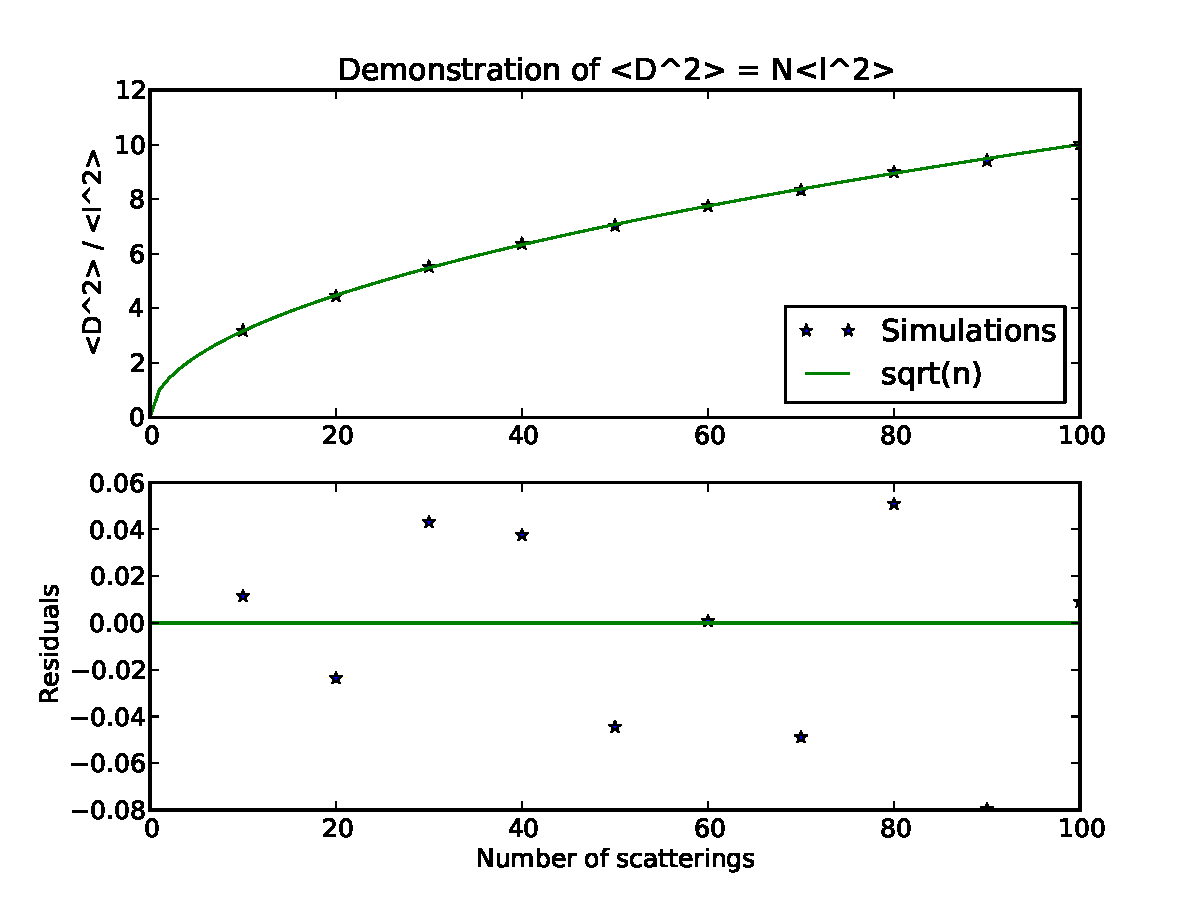
\includegraphics[width=\textwidth]{simpletest}
  \end{center}
  \caption{The 1D code was tested by verifying that for a 1D random walk, after N steps, the RMS distance from the starting point is N times the RMS step size.  Results of simulations with 10,000 photons are plotted against ${\left<d^2\right>/\left<l^2\right>=\sqrt{N}}$ (green).}
\label{fig:simpletest}
\end{figure}

To test the 1D code, I set up a simple situation to verify the property
of a one-dimensional random walk:
\begin{equation}
	\left<d^2\right> = N \left<l^2\right>
\end{equation}
where d is the net distance traveled from the original position of the
photon after N steps, with each step size drawn from the distribution $p(l|\lambda)$.

I used a constant density and an optical depth of 1000 to the edge of
the nebula to ensure that none of the photons would escape the nebula
before 10 to 100 steps were completed.  Then I ran my code for 10,000
photons, evolving them first through 10 scatterings, then 20, and so
on up to 100 scatterings.  After every 10 scatterings, I calculated
the rms distance from the center of all the photons, and compared that
to the rms step size traveled by the photons (note that this is not the
mean free path $\lambda$, but rather approximately 1.4$\lambda$, because
$\left<l^2\right>$ does not equal $\left<l\right>^2$).  Figure \ref{fig:simpletest} shows the results of this comparison.

\subsection{Test 2: Comparison of Density Profiles}

\begin{figure}[h]
  \begin{center}
     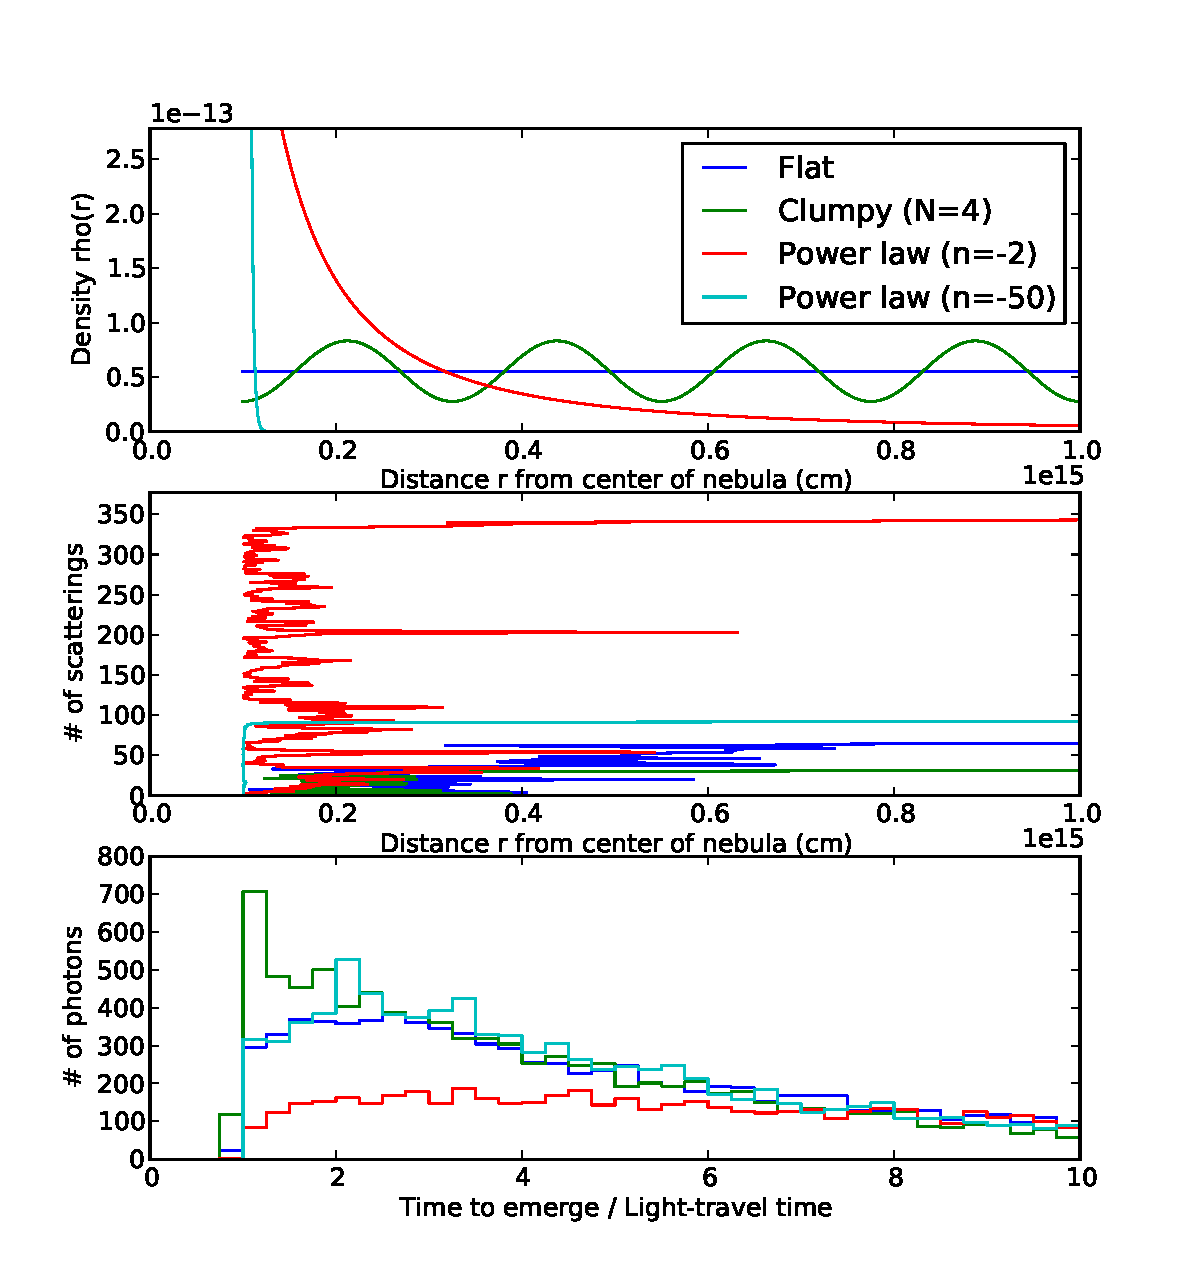
\includegraphics[width=\textwidth]{densities}
  \end{center}
  \caption{Comparison of diffusion through the different types of density profiles, each with optical depth $\tau=10$. The top panel shows the density profiles themselves.  The second panel shows a random walk of a single random photon through each profile (note: these vary consirably from trial to trial). The third panel shows the distribution of times it took for 10,000 photons to emerge from nebulae with each of the four profiles.}
\label{fig:densities}
\end{figure}

In order to understand the results below for
shock breakout, it is useful to first understand the effect of different
density profiles on diffusion time.  Figure \ref{fig:densities} shows
four different density profiles, each with optical depth $\tau=10$. The second panel shows the path of a single (randomly chosen) photon through
each of these density profiles.  These paths vary considerably from trial to trial, but the paths shown represent some common qualities: the density
profiles with the highest densities at the inner edge (where the photon starts) initially show the shortest step sizes, and thus trap the photon longer before it escapes.  However, the net distance the photon must diffuse is the scale height of the nebula, and then it can essentially move freely.  The third panel shows distributions of diffusion times for the different density profiles.  For the n=-50 power law density distribution, which has a very small scale height, the photons emerge on average earlier than for the inverse square law distribution, even though the mean free path is initially much shorter.

\subsection{Application 1: Planetary Nebulae}

\begin{figure}[h]
  \begin{center}
     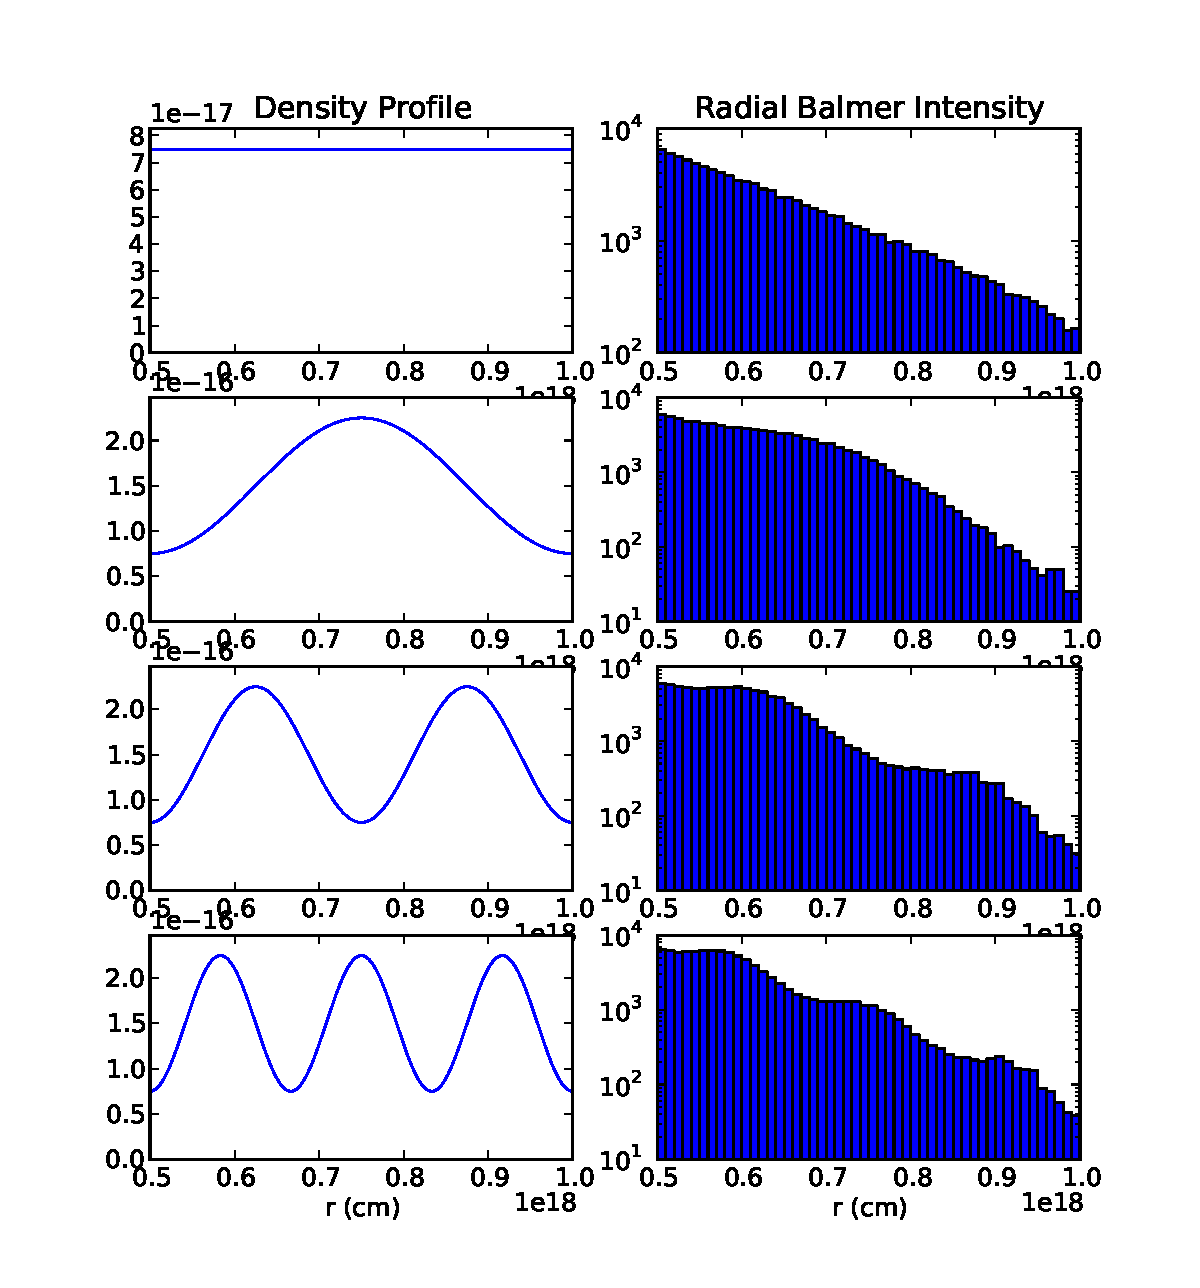
\includegraphics[width=\textwidth]{pn}
  \end{center}
  \caption{Models of the Balmer intensity from planetary nebulae with different density distributions.  The left panels show the density models (all have optical depth $\tau$=15 to Ly$\alpha$ photons), and the right
panels show the number of Balmer photons produced at each radius in a trial with 100,000 photons.}
\label{fig:pn}
\end{figure}

I used scattering as a replacement for absorption and re-emission of
Lyman-$\alpha$ photons through the processes of ionization and recombination.  I assume that the planetary nebula is optically thick to ionizing photons (which is true with even a small fraction of neutral hydrogen), choosing an arbitrary optical depth of $\tau=15$ to ensure that the photons diffuse throughout the nebula.  I compare the diffusion of photons through planetary nebulae with different numbers of ``clumps'' due to the pulsations of the parent AGB star.

When hydrogen recombines, there is some probability of recombining to a non-ground state energy level, and producing Balmer (or Paschen, etc.) photons.  Initially, I assigned a probability p=$\alpha_B/\alpha_{tot}=0.6$ (the ratio of recombination rate to $n\geq2$ to the recombination rate to all levels) of a Ly$\alpha$ photon being converted to a Balmer photon at each scattering and thus immediately escaping the nebula, which is optically thin to Balmer photons.  For Figure \ref{fig:pn}, however, I used a lower probability p=0.2 in order to give the ionizing photons more time to diffuse throughout the nebula and thus accentuate the effect of the density clumps on the Balmer intensity distribution.

I use an inner radius of 5e17 cm, and
an outer radius of 1e18 cm, to reflect a nebula that has had time to expand away from the originating star.  Since the parent star, a white dwarf, is so much smaller than the size of the cavity, essentially no photons are reabsorbed by the star.

Since the emission of Balmer photons is isotropic, the radial distribution of where Balmer photons are produced gives us an idea of what we might see for intensity versus radius when observing a planetary nebula.  Figure \ref{fig:pn} shows 4 different density profiles with different numbers of clumps, as well as the radial distribution of where Balmer photons were produced in simulations with 100,000 photons.  The clumps are observable as regions of slightly increased intensity, with the overall intensity decreasing towards the outer edge of the nebula as more ionizing photons are converted to Balmer photons.  This treatment could be improved by accounting for the decreasing ionization fraction with increasing radius, so that if the overall density remains on average constant, the density of neutral hydrogen (which ``scatters'' the ionizing photons) actually increases toward the outer edge of the nebula.

\subsection{Application 2: Shock Breakout}

\begin{figure}[h]
  \begin{center}
     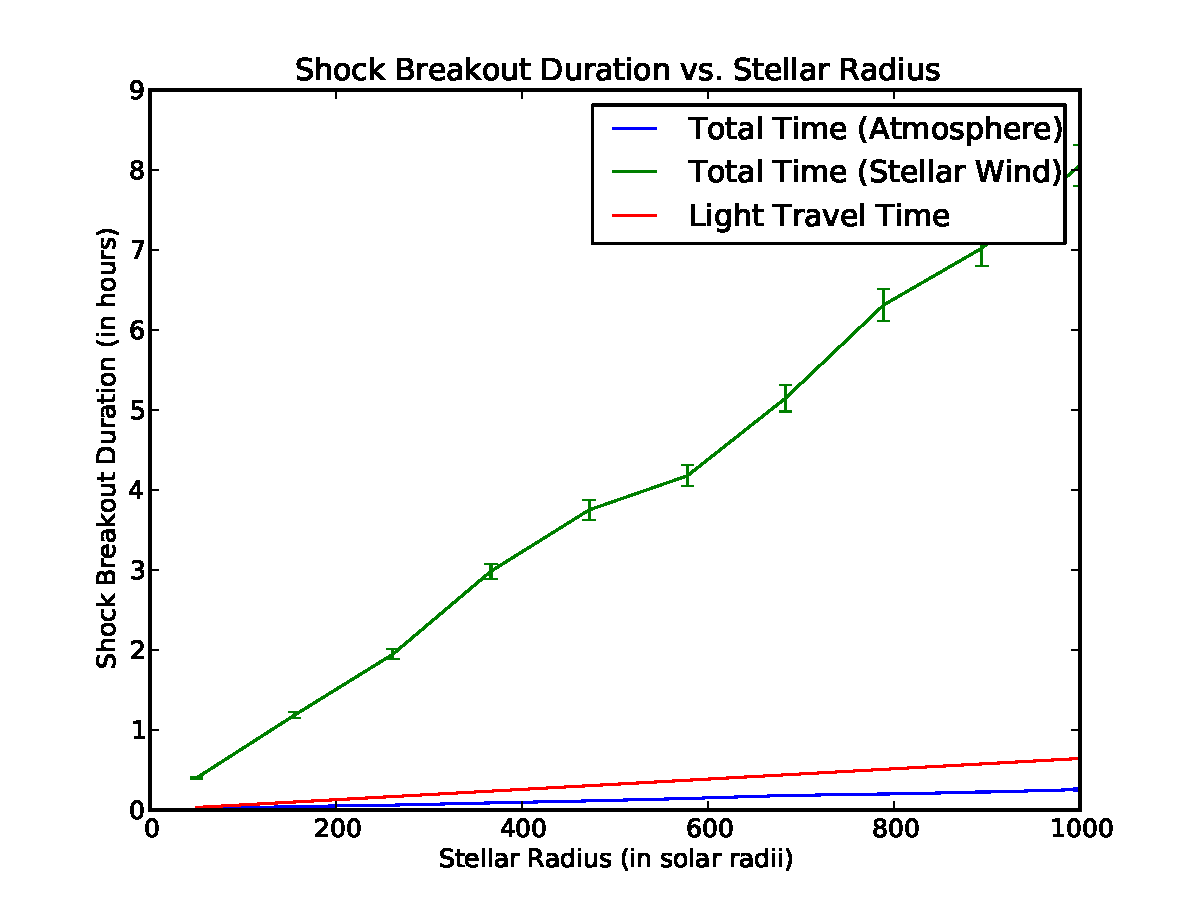
\includegraphics[width=\textwidth]{breakout}
  \end{center}
  \caption{Comparison of the contributions of diffusion time and light travel time to the duration of shock breakout, for varying progenitor radii.  In the simple model used here, $t{\propto}R_*$ in all cases.  The same optical depth $\tau=30$ was used for both the models of shock breakout occurring through a stellar atmosphere and those occurring through a stellar wind.  The error bars are a rough error estimate based on the number of photons that emerged from the star (rather than being reabsorbed by the shock front).}
\label{fig:breakout}
\end{figure}

\begin{figure}[h]
  \begin{center}
     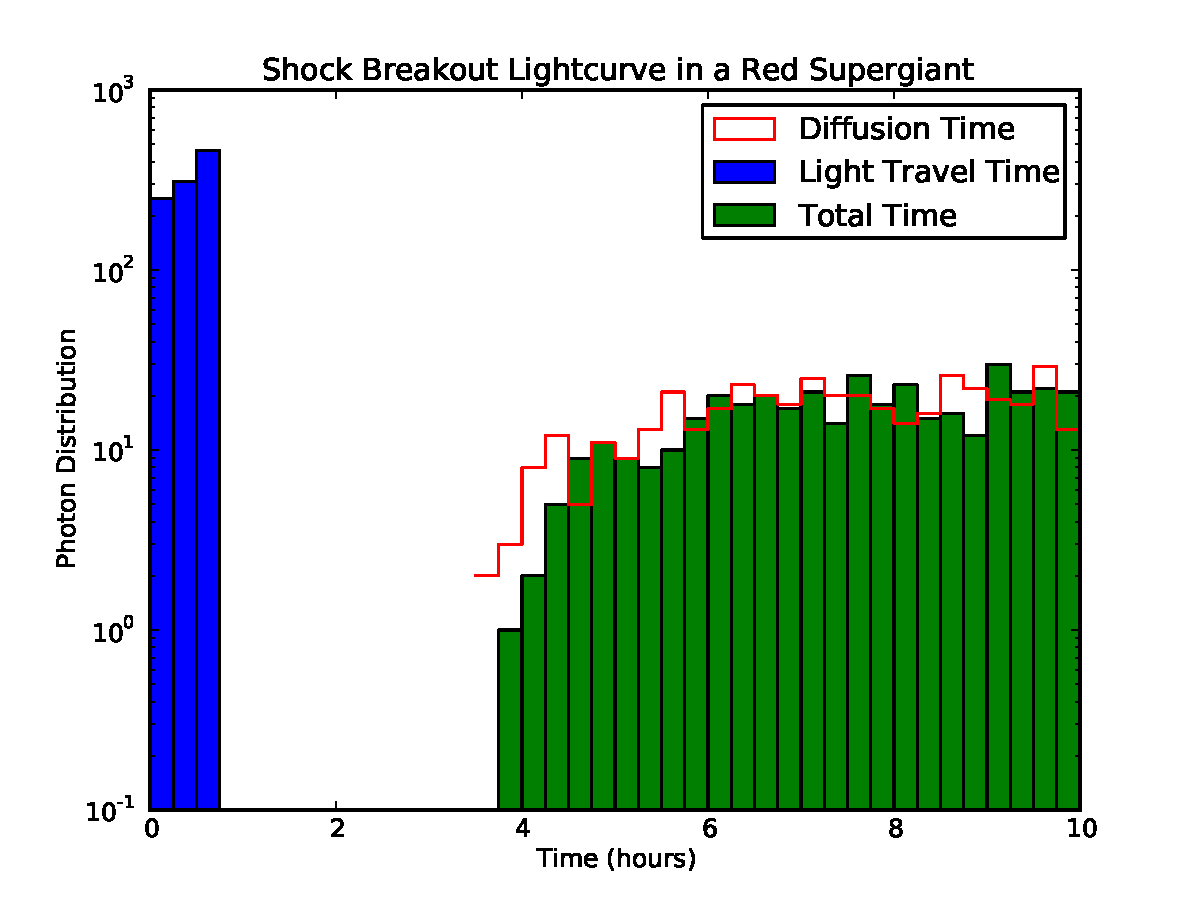
\includegraphics[width=\textwidth]{rsg}
  \end{center}
  \caption{Distribution of times for 1,021 photons to escape from a 1000$R_*$ progenitor with a stellar wind (the remaining 98,979 simulated photons were absorbed).  Red line: times to diffuse to the surface of the star.  Blue bars: time lags due to light travel time.  Green bars: total times.}
\label{fig:rsg}
\end{figure}

Shock breakout can occur in supernova progenitors ranging in size from $50R_\odot$ (blue supergiants) to $1000R_\odot$ (red supergiants).  I simulate shock breakout in stars with radii within this range.  I assume an optical depth of $\tau=30$ for the start of shock breakout, and that all the photons escape and diffuse in one burst.  Since the diffusion speed is greater than the shock speed within the region considered, I do not worry about the motion of the shock front.  I assume that photons that diffuse back onto the shock front are absorbed.  With such a high optical depth, the result is that most of the photons are absorbed.

Figure \ref{fig:breakout} shows the results for the duration of shock breakout due purely to diffusion time versus due purely to light travel time for a range of progenitor radii.  100,000 photons were used to simulate shock breakout for each stellar radius, with only 200-1000 photons escaping.  In the figure, diffusion time is shown for two types of density profiles.  The first diffusion timescale, for progenitors bounded only by their stellar atmospheres, assumes that the stellar atmosphere has a scale height of $R_*/50$, which is achieved by a power-law density profile with n=-50.  The second diffusion timescale, for progenitors with a stellar wind, assumes that the stellar wind is much faster than the escape velocity and so has an inverse square law density profile.  Even though the same optical depth was used for both cases, the stellar atmosphere has a much smaller scale height, so the diffusion time for stellar atmospheres is much shorter than that for stellar winds.  In Figure \ref{fig:breakout}, we see that light travel time determines the shock breakout duration for progenitors with only a stellar atmosphere, whereas the diffusion timescale determines the shock breakout duration for progenitors with a stellar wind. 

Figure \ref{fig:rsg} shows the details of the simulation for a $R_*=1000R_\odot$ progenitor with a stellar wind.  The figure shows the distributions of time for the photons to diffuse out, their randomly-generated light travel times (generated by simplistically assuming a random angle to the surface of the star), and the total time distribution, which is the combination of diffusion and light travel time.  The total time distribution, which has units of photons/second, shows the shape of the shock breakout lightcurve for this progenitor.  By comparing the shapes of the light travel time and diffusion time distributions, we see that the shape of the lightcurve could potentially be used to determine which timescale is more important to determining the shock breakout timescale.  If the lightcurve from a real shock breakout can be identified as light travel time-dominated or diffusion-dominated, then it can be used to infer information about the progenitor, such as its radius.

\section{What Comes Next}
This project has lots of opportunities for further exploration.  Some of the main areas are:
\begin{enumerate}
\item Integration of optical depth along the line of sight:
Currently, I sample from the mean free path at the photon's position of scattering, and then step forward the whole step length to the next scattering (equivalent to forward Euler), rather than sampling from the mean free path multiple times along the trajectory of the photon to the next scattering (similar to higher-order Runge-Kutta schemes).  One way to make this more accurate would be to generate a random optical depth, rather than a mean free path, and then integrate along the line of sight until reaching that optical depth.
\item Bias photon direction: In the example of shock breakout, where $R_*=R_{inner}$ ($R_*$ actually represents the shock front), and there is a fairly high optical depth, many of the photons scatter back into the shock front and are absorbed.  The duration of shock breakout is only determined by the photons that are not absorbed.  Since a very high fraction of photons are absorbed, it is necessary to track very many photons to obtain a statistically useful number of photons that emerge, which is computationally expensive.  One method to reduce computation time is to weight photons to have a higher probability of scattering towards the outside of the star, and later correct for the effect of these weights.
\item Modify 1D code to work for 2D:
\begin{itemize}
\item 2D density grid (types: bipolar outflow/jet, clumpy distribution, extend symmetric distributions from 1D) from $\theta=0$ to $2\pi$ (one quarter pie).
\item 2D scattering - convert from polar to rectangular coordinates, move by mean free path, convert back to polar coordinates.
\item Reflections off edges of simulated region - Rather than losing photons that pass out of the allowed $\theta$ range, reflect them back into the region.
\item Angular intensity distribution - What is the flux from the object in different directions?  What is its morphology when viewed from different directions?
\end{itemize}

\end{enumerate}

\end{document}